\documentclass{beamer}
\mode<presentation> 
{
\usetheme{Antibes}
\usecolortheme{crane}
\setbeamertemplate{footline}[page number]
}
 
\usepackage{graphicx}
\usepackage{booktabs} 
\usepackage{enumerate}
\usepackage{physics}
\setbeamerfont{caption}{size=\footnotesize}

\let\vec\mathbf
 
\title[Least Squares]{Steinhart-Hart Equation}
 
\author{Dhruv Gupta (EP17BTECH11006)\\Karthik Pagadala (EE17BTECH11049)}
\institute[IITH] 
{
Indian Institute Of Technology Hyderabad
}

\date{\today} 
 
\begin{document}
 
\begin{frame}
\titlepage
\end{frame}
 
\begin{frame}
\frametitle{Overview}
\tableofcontents 
\end{frame}

%------------------------------------------------
\section{The Equation}
%------------------------------------------------
 
\begin{frame}
\frametitle{The Equation}
\setbeamertemplate{itemize subsubitem}[circle]

\begin{itemize}

\item The Steinhart$-$Hart equation is a model of the resistence of a thermistor at different temperatures. 

\item It is defined as:
      \[
      \frac{1}{\tau} = w_{1} + w_{2} ln(R) + w_{3} {(ln(R))}^{3}
      \] where \\ $w_{1},w_{2},w_{3}$ are the Steinhart-Hart coefficients, 
      \\ $\tau$ is the temperature in Kelvin and,
      \\ $R$ is the resistence in $\Omega$
\end{itemize}
\end{frame}

%------------------------------------------------
\section{Matrix Transformation}
%-------------------------------------------------
\begin{frame}
\frametitle{Matrix Transformation}

\begin{itemize}
\item
The equation can be transformed into matrices in the following way

  \[  
  \vec{x_{1}}= \begin{bmatrix}1\\ln(R)\\{(ln(R))}^{3}\end{bmatrix} , 
  \vec{w}= \begin{bmatrix}w_{1}\\w_{2}\\w_{3}\end{bmatrix},
  \ y_{1} = \frac{1}{\tau_{1}}
  \]  
  
\item
From this, we get:

  \[
  \ y_{1} = \vec{x_{1}}^{T}\vec{w}
  \]
    

\end{itemize}
\end{frame} 

%------------------------------------------------
\begin{frame}
\frametitle{..contd.}
\begin{itemize}
\item For n$>$3: 
    \[
    \vec{y} = \begin{bmatrix}y_{1}\\y_{2}\\.\\.\\.\\y_{n}\end{bmatrix} , 
    \vec{X}^{T} = 
    \begin{bmatrix}
    \vec{x_{1}}&\vec{x_{2}}&.&.&.&\vec{x_{n}} 
    \end{bmatrix}  
    \] 
Hence, we have 
	\[
	\vec{y} = \vec{X}\vec{w}
	\]
\end{itemize}
\end{frame}
%------------------------------------------------
 %----------------
 \section{Least Squares approach}
 %------------
 \begin{frame}
\frametitle{Least Squares approach}
\begin{itemize}


\item
The Steinhart-Hart coefficients can be derived using measurements of Resistence and Temperature

\item
To get the best possible values of the coefficients, we adopted the ordinary least squares(OLS) approach.

\[f(x, \beta) = \sum_{j = 1}^m \beta_j \phi_j(x)\] 
where the function $\phi_j$ is a function of $x$

\item
Take $X_{ij}= \phi_j(x_{i})$
\end{itemize}
\end{frame}

%------------------------------------------------
\begin{frame}
\frametitle{Least Squares approach (contd.)}
\begin{itemize}
\item
The matrix X is known as the design matrix and encodes all known information about the independent variables. 
\item
It is possible to find optimal coefficients through the method of least squares using simple matrix operations. In particular, the optimal coefficients \boldsymbol{\hat\beta} as estimated by least squares can be written as follows: 
\[
\boldsymbol{\hat\beta} =( \vec{X} ^{T} \vec{X})^{-1}\vec{X}^T \vec{y}
 \] 
\item
This is the Optimum value of $\boldsymbol{\beta}$ which can be used to estimate  $y =f(x, \beta)$ with the least possible error.
\end{itemize}
\end{frame}
%------------------------------------------------

 
%-------------------------------------------
\section{Figures}
%-------------------------------------------

\begin{frame}
\frametitle{Figures}
\begin{figure}[H]
    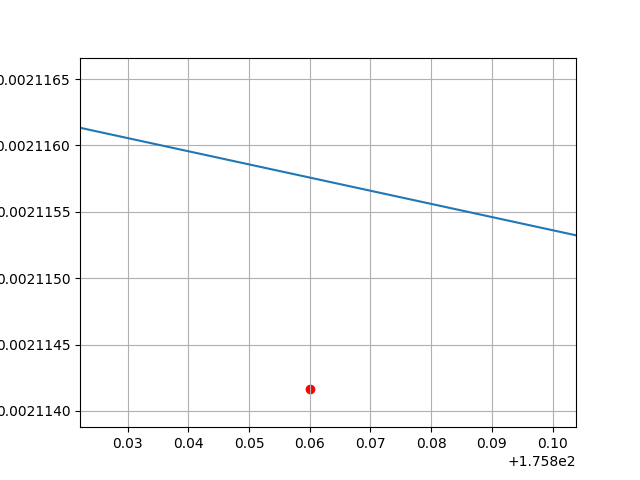
\includegraphics[width=0.7\textheight,keepaspectratio]{/home/dhruvg/Desktop/AIML/lsa/200Diff.png}
    \caption{Difference}
    \label{A3}
\end{figure}
\end{frame}
 
\begin{frame}
\frametitle{Figures}
\begin{figure}[H]
    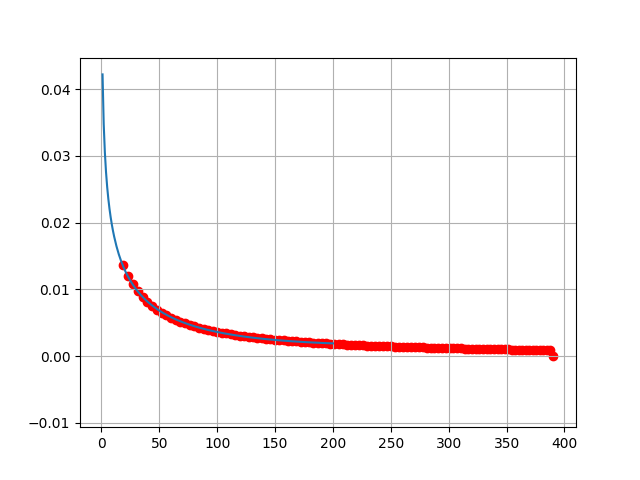
\includegraphics[width=0.7\textheight,keepaspectratio]{/home/dhruvg/Desktop/AIML/lsa/model.png}
    \caption{Model Vs Data Points}
    \label{A3}
\end{figure}
\end{frame}

\begin{frame}
\frametitle{Figures}
\begin{figure}[H]
    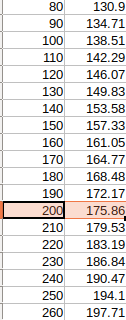
\includegraphics[height=0.8\textheight,keepaspectratio]{/home/dhruvg/Desktop/AIML/lsa/Data.png}
    \caption{Data}
    \label{A3}
\end{figure}
\end{frame}

\begin{frame}
\frametitle{Figures}
\begin{figure}[H]
    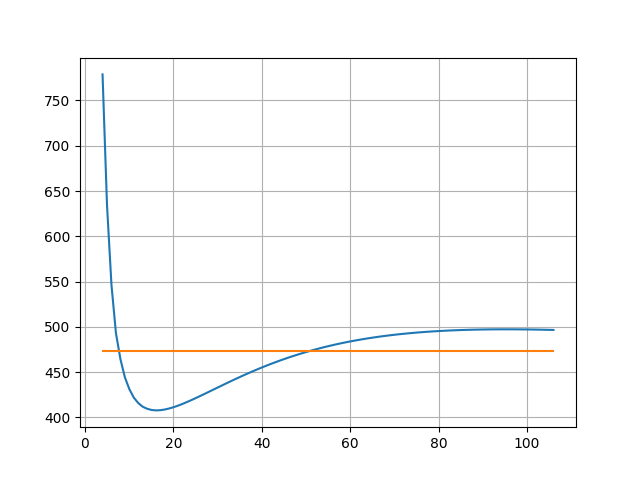
\includegraphics[height=0.7\textheight,keepaspectratio]{/home/dhruvg/Desktop/AIML/lsa/vals.png}
    \caption{Data}
    \label{A3}
\end{figure}
\end{frame}

\begin{frame}
\Huge{\centerline{.}}
\end{frame}
\end{document}
